\documentclass[11pt,a4paper]{article}

\usepackage[margin=2.2cm]{geometry}
\usepackage{setspace}
\usepackage{booktabs}
\usepackage{tabularx}
\usepackage{array}
\usepackage{amsmath,amssymb}
\usepackage{microtype}
\usepackage[hidelinks]{hyperref}
\urlstyle{same}
\usepackage{enumitem}
\usepackage{titlesec}
\usepackage{float}
\usepackage{graphicx}
\usepackage{caption}
\usepackage{xcolor}
\captionsetup{skip=5pt,font=small}

\setstretch{1.08}
\setlist[itemize]{leftmargin=1.15em,itemsep=0.12em,topsep=0.2em}
\setlist[enumerate]{leftmargin=1.15em,itemsep=0.15em,topsep=0.25em}
\titlespacing*{\section}{0pt}{0.9em}{0.35em}
\titlespacing*{\subsection}{0pt}{0.7em}{0.25em}
\titleformat{\section}{\normalsize\bfseries}{\thesection.}{0.5em}{}
\titleformat{\subsection}{\normalsize\bfseries}{\thesubsection}{0.5em}{}
\pagestyle{plain}

% Visible author tag in headings. Delete \who{...} before submission.
\newcommand{\who}[1]{\texorpdfstring{\hfill\textcolor{blue}{\textbf{[#1]}}}{}}
% Remaining work for the named owner only. Delete before submission.
\newcommand{\need}[2]{%
\par\medskip
\noindent
{\color{blue}\fbox{\parbox{\dimexpr\linewidth-2\fboxsep-2\fboxrule}{%
\textbf{[#1]} #2}}}\par\medskip}

\begin{document}
\begin{center}
{\large\bfseries Save Your Save}\\[0.35em]
{\normalsize COMP1110 Computing and Data Science in Everyday Life}\\[0.1em]
{\normalsize The University of Hong Kong \textperiodcentered\ Semester 1, 2026--2027}\\[0.45em]
{\small
\begin{tabular}{@{}lll@{}}
Vu Q.\ Nguyen \textit{(Daniel)} & 3036755728 & DP solver and policy map \\
Yerassyl Taisarinov \textit{(Yera)} & 3036459776 & Monte Carlo simulator \\
Jihun Choi \textit{(Roy)} & 3036734023 & Pok\'emon case and experiment configs \\
Yusif Seyidov \textit{(Yusif)} & 3036538850 & Analysis, figures, report assembly \\
Vivaan Kandhari \textit{(Vivian)} & 3036684400 & Synthetic data, literature, Path of Exile snapshot \\
\end{tabular}}\\[0.45em]
{\small Code and session files: \url{https://github.com/Yerasik/save-scumming}}
\end{center}
\vspace{0.4em}

%======================================================================
\section{Abstract\who{Vivian}}
At times, a game will give you a negative result, and you can replay. Trying again could possibly be worthwhile, but the minutes it consumes are minutes you can no longer spend on something better later. This paper explores the tradeoff between taking a payout in a game versus betting on the next outcome. Thus, when the game engine has a fixed series of events that all draw on one playtime budget, when should a player take what they got and when should they go again? We set it up as a dynamic programming problem, where the best action to follow depends on the current event, time remaining and the success chance. If it is not known, the model maintains a Beta belief that gets updated after every failure. We then compare the performance of the resulting policy against simpler rules, such as retrying until success or limiting retries to a constant number, via Monte Carlo simulation for 10,000 runs per strategy. In a synthetic budget experiment, at the 30-minute budget, the policy beats the best simple strategy (fixed-$k = 5$) by 18.7 reward units. In a second experiment, increasing the value of a later outcome was sufficient to reverse the policy, from retrying the early event to accepting its first outcome. We use \emph{Pok\'emon Scarlet} and \emph{Violet} as our principal worked example, and we use Path of Exile drop-rate estimates to show what uncertainty in odds looks like in practice. In general, one will only retry if the expected gain is greater than the value of saving that time for later opportunities.

\need{Vivian}{Tighten to the course word limit if needed. Keep the 18.7 gap, the later-prize reversal, Pok\'emon, and Path of Exile.}

%======================================================================
\section{Introduction\who{Vivian}}
If the player receives a nasty reward, they have 40 seconds left. Retrying the current encounter takes 20 seconds, and getting to the next encounter takes 30. Retrying therefore spends the time that would have paid for the next encounter, even though 40 seconds is enough for one more attempt now. If they take the poor reward and move on, they can still make it.

This trade-off is difficult to notice when save-scumming, that is, loading a saved game to try for a better outcome, as the player sees the current result right away, while the cost of trying again may not be apparent until later. The same retry can shut down other options as the deadline approaches. If the odds of success are unknown, repeated failures can also alter the perceived promise of the next attempt.

So we ask: when should a player accept a bad outcome or retry if several encounters share one playtime budget? We focus on fixed-order encounters, so players have the option to spend more time on the current event or move on. We investigate the conditions under which it pays to look ahead and when a simple policy such as stopping after a specified number of retries is good enough.

We report three tests, named after the hypotheses in the project plan rather than the folder letters A--D. \textbf{H1} asks whether looking ahead helps most when the clock is tight but not empty. \textbf{H3} asks whether a valuable later event can make retrying an earlier one a mistake. \textbf{H5} asks whether, when the odds are unknown, a retry cap can beat retrying until success. The repository also has probability and retry-cost sweeps (B and C); they are not in this report, because they do not test those three claims. There is no H2 or H4 here: those were never lead hypotheses. Naming the runs H1, H3 and H5 keeps each table tied to a claim instead of a file name.

%======================================================================
\section{Background and context\who{Vivian}}
Save-scumming means saving just before a random event and reloading until the result is good enough. It is how players chase the right nature on a legendary Pok\'emon, a good loot roll, or a passed dialogue check. A related habit is farming: repeating a boss or a map for a rare drop. In both cases one attempt is cheap but a long string of them is not, so we use ``retry'' and ``reload'' to mean the same thing.

For one event on its own, deciding whether to retry is easy: compare the chance of success and the reward against the time. It gets harder when several events come in a row and share one playtime budget. Every retry on the current event uses time that could go to a later one. Chasing a 5\% roll can make sense when nothing valuable is left, and be a poor use of the same minutes when a better event is still ahead. So the same failed roll can call for different actions depending on where the player is in the session.

Players rarely set a budget for themselves, but real life does it for them: class the next morning, a limited-time in-game event, the end of an online season. Anything not reached before then is missed. We call this the limited-playtime setting, and it is the main focus of this report. A second complication is that the odds are not always known. Pok\'emon natures follow a published rule (1 in 25 each). Many drop rates in Path of Exile are only community estimates, so a player who keeps failing should start to doubt the estimate.

%======================================================================
\section{Problem definition\who{Vivian}}
A session is a fixed sequence of $n$ events played in order, with a total time budget of $T$ seconds. Event $i$ has:
\begin{itemize}
\item a success chance $p_i$ per attempt. If the odds are not published, the player holds a $\mathrm{Beta}(\alpha_i, \beta_i)$ belief about $p_i$ instead;
\item a good reward $g_i$ and a bad reward $b_i$, with $g_i > b_i$;
\item a retry time $c_i$ (seconds per extra attempt);
\item a travel time $f_i$ to reach the next event (the last event has $f_n = 0$).
\end{itemize}

The first attempt at an event is free. If it fails, the player has two options: accept $b_i$ and move on, or spend $c_i$ seconds to try again. If time runs out before the player reaches an event, that event is lost. The goal is to choose, after every failure, whether to accept or retry so that the expected total reward over the session is as large as possible.

We assume attempts are independent, there is one target outcome per event, the order of events is fixed, and success or failure at one event does not change what comes later. Rewards are fixed points within a session, not values that change during play. We do not model branching stories, RNG manipulation, or anything that needs access to a game's code.

\need{Vivian}{Add one sentence that $e_i = 0$ and $h_i = 0$ in every reported session (no entry cost; a reload discards the bad result).}

%======================================================================
\section{Literature review and research gap\who{Vivian}}
\subsection{Existing literature}
Save-scumming is when you reload a saved game to get a different outcome. Farmer, Kelly and Jones-Rincon~\cite{farmer2025} look at why players do this using self-determination theory to explore their motivations. Their study helps explain why reloading is a meaningful part of the way some players play games. Our project answers a different question: when is it worth the time to try again, given a player is willing to reload?

One way to think of this decision is to consider research on algorithm restarts. Luby, Sinclair and Zuckerman~\cite{luby1993} investigate the gain from restarting a randomised algorithm to reduce the expected time to get an answer. Lorenz~\cite{lorenz2016} investigates the impact of restart strategies on the probability of deadline satisfaction. Both works show why it matters how long you spend on another try. But they are built to do one computational task, while a player can accept a bad outcome and move on to another encounter.

The decision also concerns costly search. Weitzman~\cite{weitzman1979} considers the point at which it is worthwhile to search for another uncertain reward, and when it is better to stop. This is useful for thinking about whether the time taken is worth the probability of a better roll. In Weitzman's model, the decision maker has the option to inspect any opportunity next. In our setting, encounters are processed in a fixed order, so the question is whether to stay at the current encounter or move to the next one.

Another challenge is knowing when the odds are unknown. DeGroot~\cite{degroot2004} gives a framework for updating beliefs based on observations and making decisions based on the beliefs. Russo et al.~\cite{russo2018} explain that an action can provide both immediate reward and information that can be used to make better decisions in the future. In our project, a failed attempt is time-consuming and gives information about the unknown success probability. We model that uncertainty with a Beta distribution. Failures can decrease the player's estimate of success, but the underlying probability does not change.

The other two sources connect these ideas to the method of the project. Kleinberg, Slivkins and Badanidiyuru~\cite{badanidiyuru2018} consider the problem of learning and collecting rewards in the setting of actions consuming a limited resource. That work helps to explain the value of an attempt by noting what else the player might do with the same amount of time. Dynamic programming appraises decisions with consequences that affect subsequent decisions~\cite{sargent2025}. The framework that they gave allows us to compare retrying now versus moving on with more time left.

\subsection{Research gap}
Each strand of work above covers part of our problem, but none covers all of it. Save-scumming research~\cite{farmer2025} studies why players reload, not whether a reload is worth the time. Restart models~\cite{luby1993,lorenz2016} ask when to retry, but for a single task with nothing else to move on to. Weitzman's~\cite{weitzman1979} search model lets the searcher pick any option next, whereas a player has to follow the game's route, travel time included. Bandits with Knapsacks~\cite{badanidiyuru2018} combines learning with a limited budget, but it has no fixed order of named events.

In the work we reviewed, we did not find a model that splits one real-time budget across several game events in a fixed order, gives an accept-or-retry decision for each, and still works when the odds are unknown and have to be learned from failures. Our project combines dynamic programming with a Beta belief to fill that gap. It also asks a practical question that the theory alone does not answer: how much better is the best policy than the simple rules players actually use?

\need{Vivian}{Add any extra sources you want cited, and check author order on Badanidiyuru, Kleinberg and Slivkins (2018). Finish the reference list in Section~\ref{sec:refs}.}

%======================================================================
\section{Technical design, analytical approach and methodology}
\subsection{Technical design\who{Vivian}}
The project is a Python prototype, not an app. The code, session files, policies and experiment outputs are in the GitHub repository \url{https://github.com/Yerasik/save-scumming}. It has four parts, linked by plain files so each person could work on their own part:
\begin{itemize}
\item \textbf{Session files (JSON).} Each session lists its events with $p$ (or $\alpha$ and $\beta$), $g$, $b$, $c$, $f$, and the budget $T$. The format was fixed early, so synthetic sessions and the Pok\'emon session use exactly the same fields.
\item \textbf{Solver (\texttt{dp/}).} Reads a session and writes a policy file: for every event, time left and failure count, whether to retry or accept.
\item \textbf{Simulator (\texttt{sim/}).} Plays the session event by event with real random rolls under a named strategy, and records reward, number of reloads and time spent reloading. The simulator never solves anything. For the DP strategy it simply looks up the policy file.
\item \textbf{Analysis (\texttt{analysis/}).} Reads the simulator's CSV output and draws the figures.
\end{itemize}
Keeping the solver and the simulator separate matters. If the DP's predicted value and the simulator's result agree, that is evidence both are correct, because they were written independently.

\subsection{Analytical approach\who{Vivian}}
\label{sec:dp}
After any decision, the rest of the problem is fully described by three numbers: the current event $i$, the seconds left $t$, and the number of failures $k$ at this event so far. Let $V(i,t,k)$ be the best expected reward from here on, $W(i,t,k)$ the same value just after a failure, and $N(i,t)$ the value of moving on to the next event:
\begin{align}
N(i,t)
&=
\begin{cases}
V(i+1,\, t-f_i,\, 0)
& \text{if } t \ge f_i \text{ and there is a next event,}\\
0 & \text{otherwise,}
\end{cases}
\label{eq:N}\\[0.3em]
W(i,t,k)
&=
\max\bigl\{
b_i + N(i,t),\;
V(i,\, t-c_i,\, k+1)
\bigr\},
\quad\text{retry only if } t \ge c_i,
\label{eq:W}\\[0.3em]
V(i,t,k)
&=
q_i(k)\,(g_i + N(i,t))
+ \bigl(1-q_i(k)\bigr)\, W(i,t,k).
\label{eq:V}
\end{align}
In words: with probability $q$ the attempt succeeds and the player takes $g$ and moves on. Otherwise they pick the better of accepting $b$ and moving on, or paying $c$ seconds to try again with one more failure on record. The value of the whole session is $V(1,T,0)$.

The term $q_i(k)$ is the player's current estimate of the success chance:
\begin{itemize}
\item \textbf{Known odds:} $q_i(k) = p_i$, which never changes.
\item \textbf{Unknown odds:} $q_i(k) = \alpha_i / (\alpha_i + \beta_i + k)$, the Beta posterior mean after $k$ failures. For example, $\mathrm{Beta}(1,49)$ starts at a 2\% belief and falls to 1\% after 50 failures. The true chance does not change, but the player's estimate of it does, so retrying gets less attractive with each failure.
\end{itemize}

We fill the table backwards over events (last event first) and upwards over time, in whole seconds. There are $n \times T \times K$ states, where $K$ is the most failures that fit in the budget. Known odds only need $k = 0$, and even the largest sessions solve in seconds. Two small choices: when retrying and accepting are exactly equal, the solver accepts, and a retry is allowed when $t \ge c_i$, matching the simulator. The output is a policy map, which we keep in full because the best action can switch more than once as time runs out.

As a simpler reference point, we also use the reward-per-second rule from our project plan: with no deadline and an outside value of time $\rho$, retrying event $i$ is worth it exactly when
\[
q_i(k)\,(g_i - b_i) \ge \rho\, c_i.
\]
This rule is what a player would use if missing later events were not a risk.

\need{Vivian}{You own the $\rho$-baseline: state the value of $\rho$ used (or that efficiency-greedy used cutoff $0.10$). Also check that equations~\eqref{eq:N}--\eqref{eq:V} match what you meant; every session in this report has $h_i = 0$.}

\subsection{Datasets\who{Yera}}
The solver and the simulator take the same session files. Three kinds of session appear in this report.

\textbf{Synthetic factor sweeps.} H1 is an 8-event session whose only changing field is the time budget $T$. H3 is a two-event session whose only changing field is the later event's good reward (or that event is removed). H5 is a two-event session whose only changing field is the prior on the first event. These files exist so that one named factor can be moved at a time.

\textbf{Pok\'emon Scarlet / Violet (main case).} A four-shrine postgame route with known odds. Each shrine is a nature hunt at $p = 0.08$ (2 natures out of 25). Retry and travel times are means from public videos. Budget $T = 60$ minutes. Rewards are stated preferences $(20, 30, 20, 30)$, not market prices.

\textbf{Path of Exile contrast.} A session named after the regular Searing Exarch encounter. The rare unique is given a $\mathrm{Beta}(1,49)$ belief (2\% mean, from a dated community snapshot). Retry and travel times match the H5 sessions; they are not measured from Path of Exile footage. This file is an illustration of unknown odds, not a farming calculator.

Every result below is 10,000 Monte Carlo sessions per strategy. Seeds are $0$ through $9{,}999$ and are reused across strategies. Mean reward is reported with a 95\% interval (mean $\pm 1.96$ SE). When two strategies are compared, the difference is paired on those shared seeds.

\need{Roy}{Insert the shrine table: event, target natures, $p$, mean retry $c$, mean travel $f$, and how the video timestamps were averaged (3 retry videos and 2 travel videos per event). Dropped events (shiny-locked, nature-locked) in one short list.}

\need{Vivian}{Path of Exile snapshot (you own this): date 2026-11-05, league Mercenaries 3.26, source of the 2\% figure, and that prices were left unobserved.}

\subsection{Methodology\who{Vivian}}
\label{sec:method}
We compare the DP policy with the simple rules a real player might follow:

\begin{table}[H]
\centering
\caption{Strategies compared by the simulator after a failed roll.}
\small
\begin{tabularx}{\textwidth}{@{}l X@{}}
\toprule
\textbf{Strategy} & \textbf{Rule} \\
\midrule
Never reload & Always accept. \\
Always reload & Retry until success, while $\mathrm{time\_left} \ge c_i$. \\
Fixed-$k$ & At most $k$ attempts per event ($k = 2,3,5$), counting the free first attempt. \\
Reward-greedy & Retry only the highest-reward event, keeping enough time to reach the last event. \\
Efficiency-greedy & Retry while $p(g-b)/c$ is above a cutoff ($0.10$ here), keeping enough time to reach the last event. For Beta events the rate uses the prior mean, not the hidden $p$. \\
DP & Follow the policy map. The simulator does not re-solve the dynamic program. \\
\bottomrule
\end{tabularx}
\end{table}

Each experiment changes one factor and keeps everything else fixed. We name them H1, H3 and H5 after the three lead hypotheses, not A, B, C, D after the config folders:
\begin{itemize}
\item \textbf{H1 (time budget).} An 8-event session played with $T = 10, 20, 30, 60$ and $120$ minutes. Is the DP's advantage largest at moderate time pressure, and near zero if the budget is tiny or huge?
\item \textbf{H3 (later prize).} An early event ($p = 0.1$, $g = 10$) followed by a rare, slow later event ($p = 0.05$) that is either removed or worth $10, 20, 40, 80$ or $160$. Is there a later reward large enough that the DP stops retrying the early event?
\item \textbf{H5 (unknown odds).} A rare drop with the same 2\% average chance in every session, either known or held as $\mathrm{Beta}(20,980)$, $\mathrm{Beta}(1,49)$ or $\mathrm{Beta}(0.2,9.8)$, followed by a later known event. When the odds are unknown, can a retry cap beat retrying until success? Because the simulator's fixed-$k$ rule caps every event, we also tested caps on the rare drop alone (1 to 90 attempts), so that the comparison is about uncertainty and not about giving up on the later event too.
\end{itemize}

Every strategy is played on the same 10,000 random seeds. That way, differences between strategies come from the strategies, not from luck. In the unknown-odds sessions, the simulator draws one true success chance per seed from the Beta prior and keeps it for every retry, which matches what the DP assumes. We report mean reward with 95\% confidence intervals, and use paired differences on the shared seeds when two strategies are close.

We checked the engine three ways before trusting the results:
\begin{enumerate}
\item The simulated mean reward of the DP policy matched the solver's predicted value in every session, within 2.5 standard errors (within 1.2 for all four H5 sessions).
\item The average number of tries until a success matched $1/p$, as it should for independent rolls.
\item Automated tests cover the solver, the simulator and the input files, and all of them pass.
\end{enumerate}

%======================================================================
\section{Simulation engine and experiment results}
\subsection{How a session is played\who{Yera}}
\label{sec:sim}
The simulator walks the event list in order and spends a shared clock, starting at $T$ seconds. It does not solve a dynamic program. For the DP strategy it only looks up the written policy file after each failure.

The first attempt at a reached event is free. A success adds $g_i$ and the player pays travel $f_i$ to the next event. A failure is then a choice: take $b_i$ and move on, or pay $c_i$ seconds, throw away the bad roll (retained failure reward is 0 in every session here), and roll again. If the clock cannot pay $f_i$, later events are never reached and score 0. If the clock cannot pay $c_i$, a retry is treated as accept.

Known-odds events use the published $p$ on every roll. Beta events draw one hidden success chance per $(\mathrm{seed},\mathrm{event})$ from $\mathrm{Beta}(\alpha,\beta)$ and keep that chance for every retry of that seed. Strategies that share a seed therefore face the same luck and the same hidden $p$. That is what makes ``DP beat always by $X$'' a statement about the rule, not about a luckier sample.

Each row of the output CSV is one (session, strategy, seed) playthrough: total reward, number of reloads, and seconds spent reloading.

\subsection{H1: time budget\who{Yera}}
\label{sec:H1}
Question: when does looking ahead beat a simple habit? Only $T$ changes: 10, 20, 30, 60, and 120 minutes. The eight events stay fixed.

H1 says the DP's edge over the best simple rule is largest at moderate pressure and near zero if the budget is tiny or huge.

\begin{table}[H]
\centering
\caption{H1, 10,000 shared seeds. Mean reward $\pm$ 95\% CI. The last column is the paired difference DP minus the best simple rule.}
\label{tab:H1}
\small
\begin{tabular}{@{}l l r r r@{}}
\toprule
\textbf{Budget} & \textbf{Best simple rule} & \textbf{DP} & \textbf{Best simple} & \textbf{DP $-$ best} \\
\midrule
10 min  & efficiency-greedy & $67.0 \pm 0.5$  & $66.9 \pm 0.5$  & $0.1 \pm 0.2$ \\
20 min  & efficiency-greedy & $91.5 \pm 0.5$  & $82.8 \pm 0.3$  & $8.6 \pm 0.5$ \\
30 min  & fixed-$k = 5$     & $107.5 \pm 0.6$ & $88.7 \pm 0.6$  & $\mathbf{18.7 \pm 0.6}$ \\
60 min  & always            & $137.9 \pm 0.7$ & $127.8 \pm 1.0$ & $10.1 \pm 0.5$ \\
120 min & always            & $158.5 \pm 0.4$ & $156.4 \pm 0.5$ & $2.1 \pm 0.2$ \\
\bottomrule
\end{tabular}
\end{table}

That is what H1 predicts. At 10 minutes there is almost no room to spend extra retries, so efficiency-greedy already matches DP (the $0.1$ gap is inside the interval). At 30 minutes the gap is $18.7$. At 120 minutes always-reload is almost as good, because later events are no longer at risk.

The best simple rule also changes with $T$: efficiency-greedy when time is tight, a retry cap in the middle, always-reload when time is loose. No single habit wins every budget. The DP switches between those habits by itself.

\begin{figure}[H]
\centering
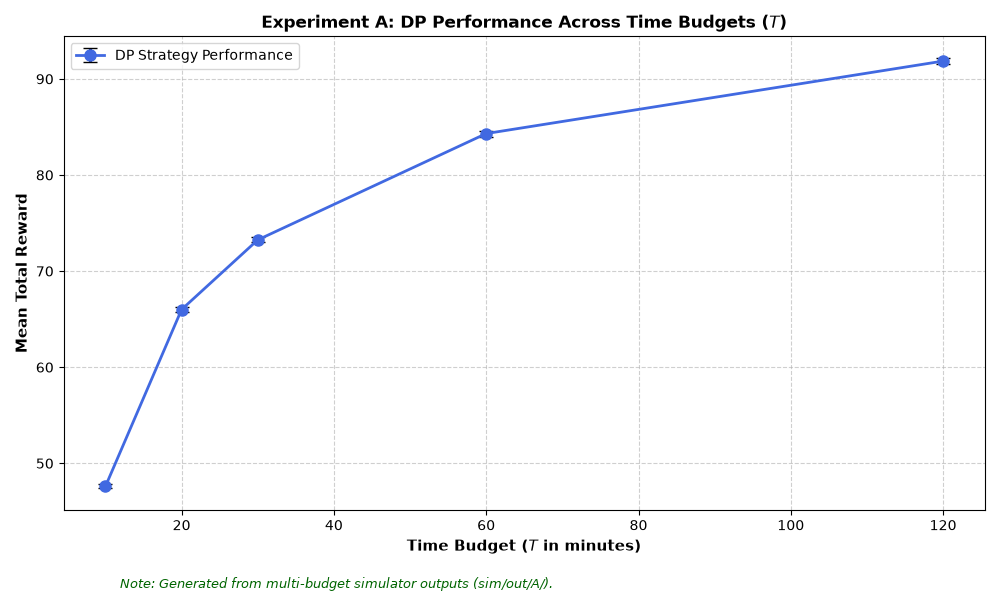
\includegraphics[width=0.92\textwidth]{analysis/experiment_a_chart.png}
\caption{H1: mean reward against time budget. Error bars are 95\% CIs.}
\label{fig:H1}
\end{figure}

\need{Yusif}{You own the figures: replace Fig.~\ref{fig:H1} if the analysis script changes axis labels. Keep the paired-difference story in Table~\ref{tab:H1}.}

\subsection{H3: a later prize\who{Yera}}
\label{sec:H3}
Question: is there a later reward large enough that the DP stops retrying an earlier event?

The first files for this sweep could not answer this. The later event had $p = 0.5$ and a 10-second retry, so it was almost always won in a few tries. Raising its reward from 8 to 80 did not change the early policy. The rebuilt H3 sessions keep the hard early event from the toy ($p = 0.1$, $g = 10$, $c = 20$\,s) and make the later event rare and slow ($p = 0.05$, $c = 30$\,s), with $T = 600$\,s. Only the later good reward changes: removed, 10, 20, 40, 80, 160.

From a full budget, the DP's planned retries on the early event are:

\begin{table}[H]
\centering
\caption{H3 policy: planned retries of the early event from a full budget.}
\label{tab:H3policy}
\small
\begin{tabular}{@{}l rrrrrr@{}}
\toprule
Later reward & removed & 10 & 20 & 40 & 80 & 160 \\
\midrule
Early retries (DP) & 30 & 30 & 30 & 18 & 0 & 0 \\
\bottomrule
\end{tabular}
\end{table}

At 80 and 160 the policy gives up on the early event entirely. That is H3 on the policy map.

\begin{table}[H]
\centering
\caption{H3, 10,000 shared seeds. Mean reward.}
\label{tab:H3}
\small
\begin{tabular}{@{}l rrrrrr@{}}
\toprule
 & removed & 10 & 20 & 40 & 80 & 160 \\
\midrule
DP             & 9.6 & 14.5 & 19.4 & 29.2 & 52.7 & 104.2 \\
Always reload  & 9.6 & 14.5 & 19.4 & 29.1 & 48.5 & 87.4 \\
Reward-greedy  & 9.6 & 10.0 & 14.0 & 26.9 & 52.7 & 104.2 \\
\bottomrule
\end{tabular}
\end{table}

While the later prize is small, DP and always-reload are the same: keep retrying the early event. Once the later prize is 80 or more, DP matches reward-greedy instead, and always-reload loses $4.1$ (80) and $16.8$ (160) because it burns the clock on the early 10-point event. No single simple rule wins the whole sweep. The DP is the rule that switches.

\begin{figure}[H]
\centering
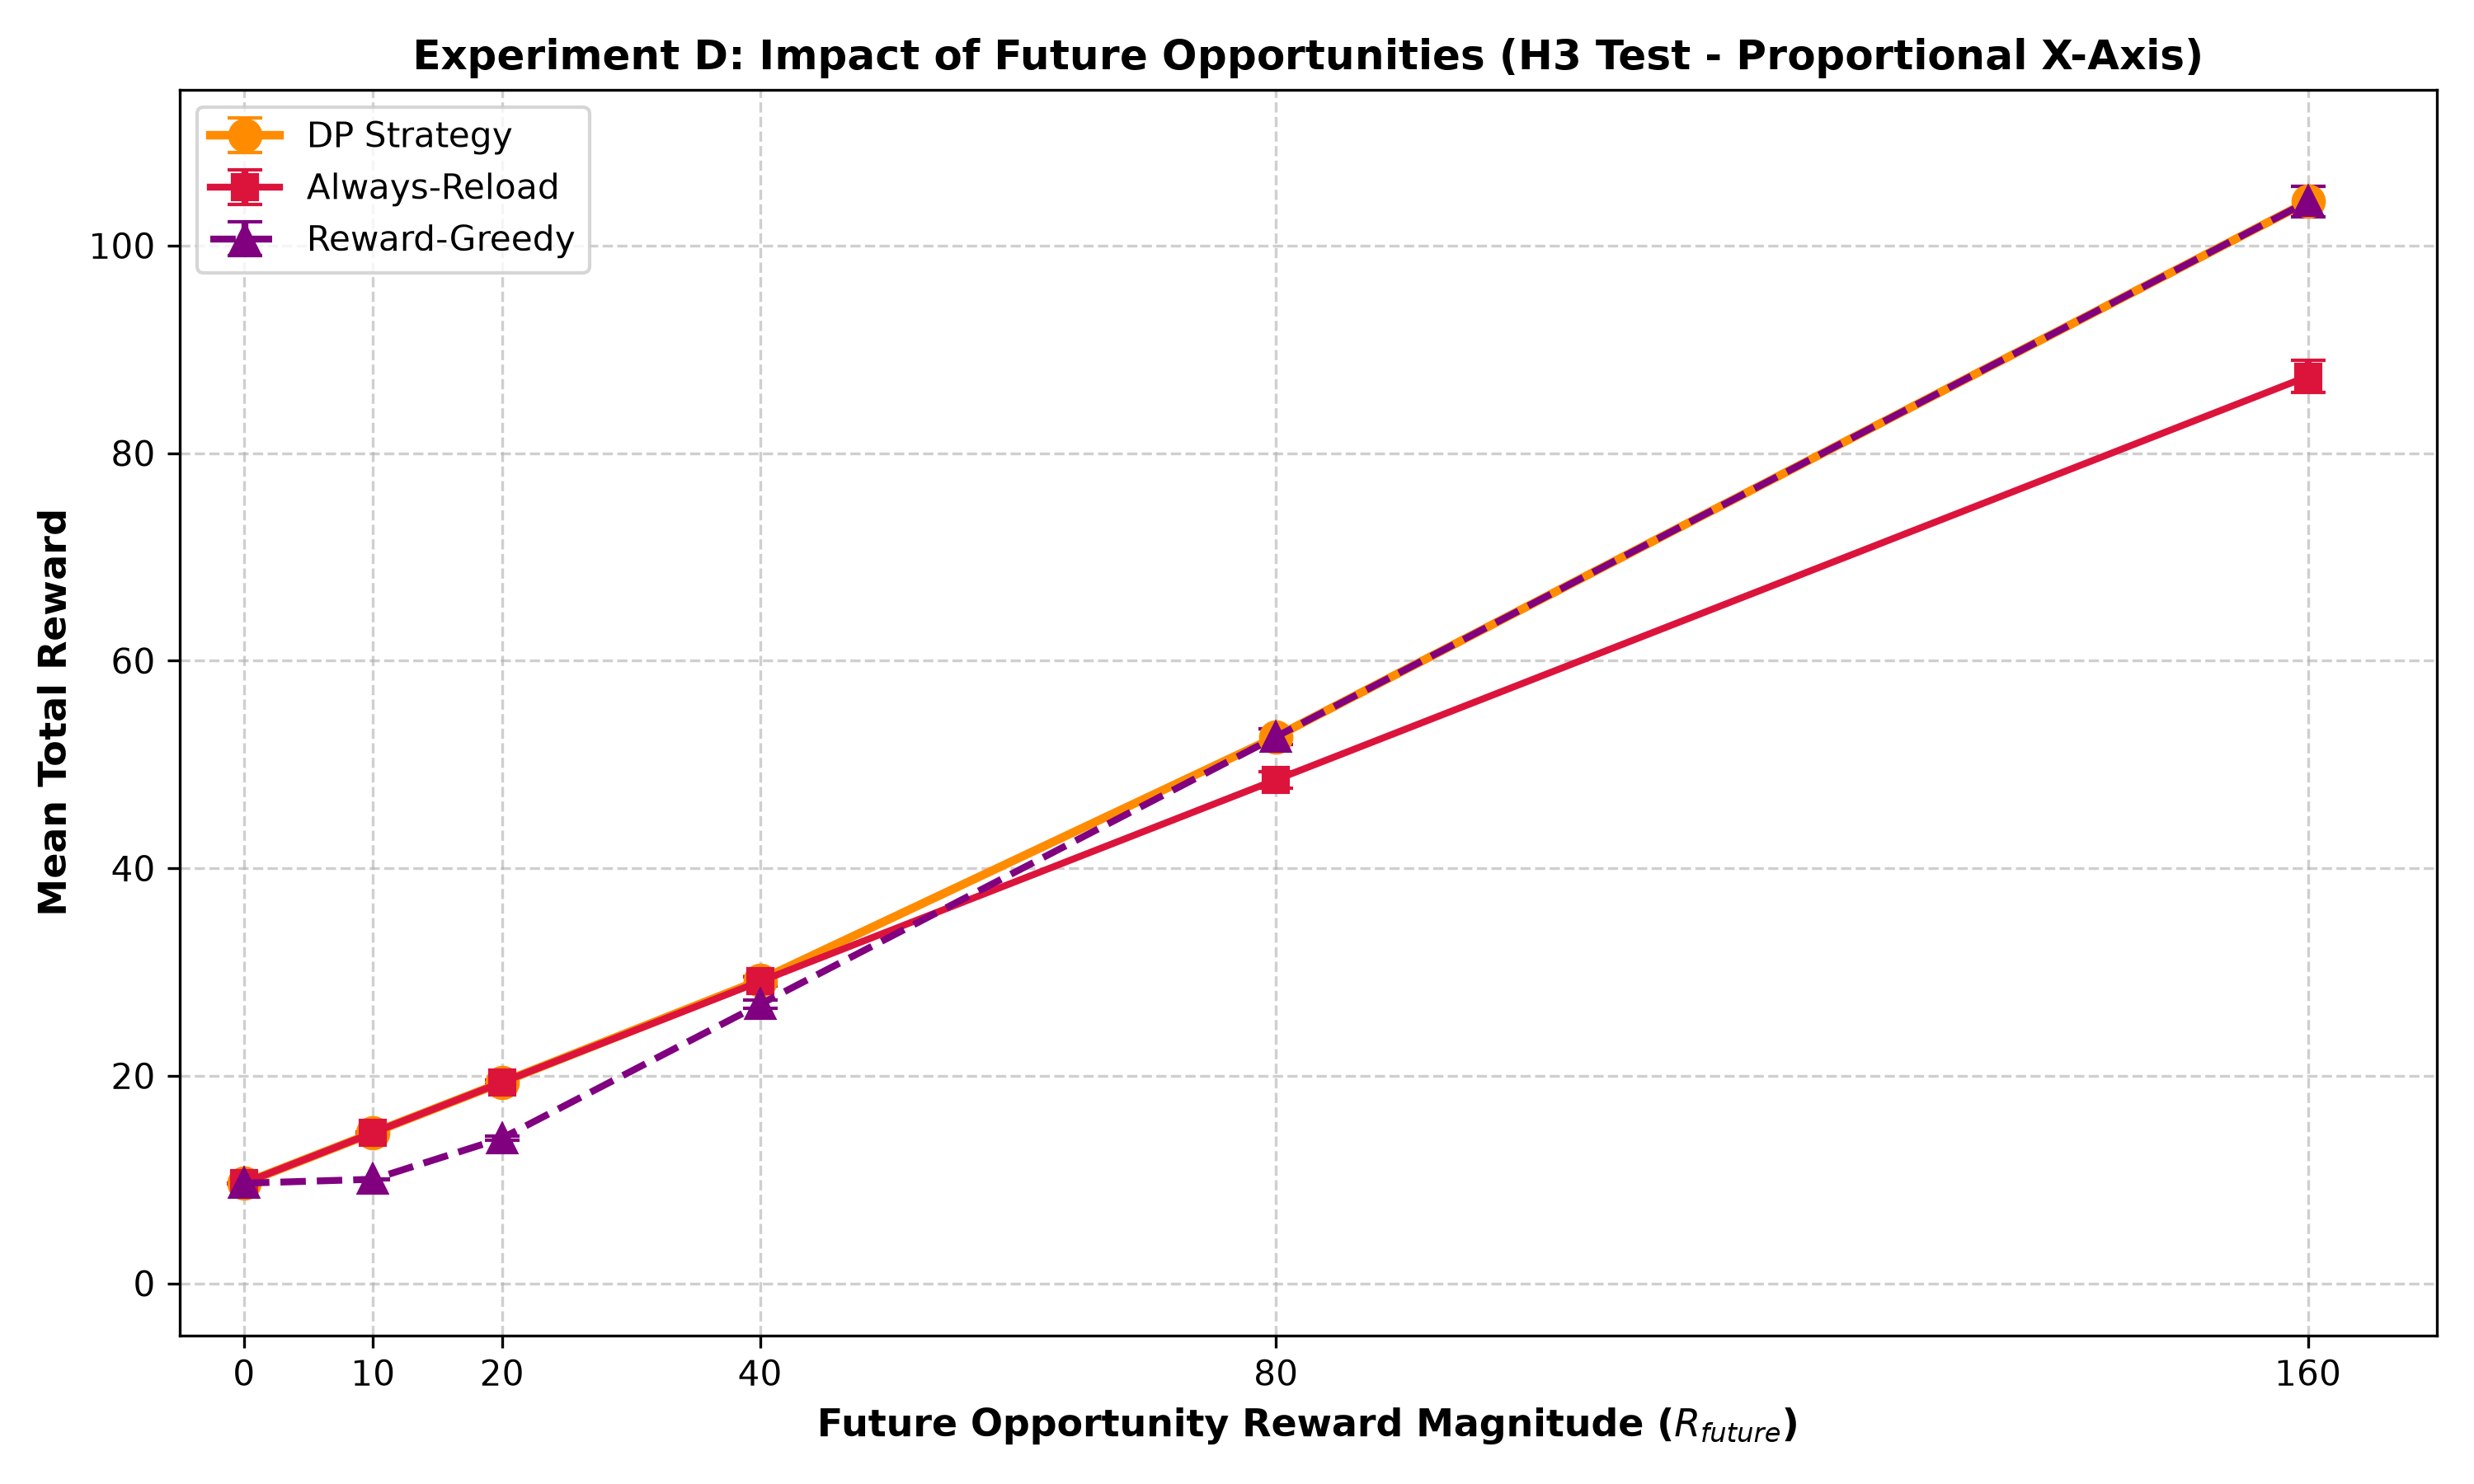
\includegraphics[width=0.92\textwidth]{analysis/experiment_d_chart.png}
\caption{H3: mean reward as the later prize changes.}
\label{fig:H3}
\end{figure}

\subsection{H5: unknown odds\who{Yera}}
\label{sec:H5}
Question: when the odds are unknown, can a retry cap beat retry-until-success?

Four sessions share the same 2\% mean on a rare drop, then a later known event that competes for the same 30-minute clock. The four beliefs are: known $p = 0.02$, $\mathrm{Beta}(20,980)$ (strong), $\mathrm{Beta}(1,49)$, and $\mathrm{Beta}(0.2,9.8)$ (weak). Retry time is 20 seconds. An earlier file used 60 seconds, and the DP never retried, so a cap and always-reload would have looked the same for the wrong reason.

The simulator's $\mathrm{fixed}\text{-}k = 2,3,5$ rule is not a fair test here. It caps every event. At $p = 0.02$ those caps barely use the budget and score about 13--32 against about 150. That gap is ``gave up on the later event too,'' not ``handled uncertainty.'' The comparison that belongs in this section caps only the rare drop, keeps travel to the next event, lets the later event retry until success, and sweeps the cap from 1 to 90 attempts.

\begin{table}[H]
\centering
\caption{H5, 10,000 seeds. Always-reload vs the best cap on the rare drop only vs DP. The ``cap $-$ always'' column is paired.}
\label{tab:H5}
\small
\begin{tabular}{@{}l r r r r@{}}
\toprule
\textbf{Belief} & \textbf{Always} & \textbf{Best cap (attempts)} & \textbf{Cap $-$ always} & \textbf{DP (sim)} \\
\midrule
Known $p = 0.02$     & 152.0 & 153.8 (75) & $+1.8$  & 153.8 \\
$\mathrm{Beta}(20,980)$ & 149.1 & 151.6 (75) & $+2.5$  & 151.6 \\
$\mathrm{Beta}(1,49)$   & 118.1 & 133.6 (60) & $+15.6$ & 134.1 \\
$\mathrm{Beta}(0.2,9.8)$& 69.4  & 114.1 (30) & $+44.7$ & 114.1 \\
\bottomrule
\end{tabular}
\end{table}

A cap helps a little when the odds are known, because the later event still needs time: always-reload keeps hitting the 2\% drop until the clock forces it out (H3 again). A cap helps a lot when the odds are uncertain, and the extra gain grows as the prior gets weaker ($+2.5$, then $+15.6$, then $+44.7$, against $+1.8$ when $p$ is known). The best cap also shortens ($75 \to 60 \to 30$), which is where the DP gives up on the policy map.

On this one-uncertain-event setup, the best fixed cap is as good as the DP (within $0.5$). The DP's value is that it finds that $N$ from the belief. A player who picks $N$ by hand has to already know roughly how unsure they are.

\begin{figure}[H]
\centering
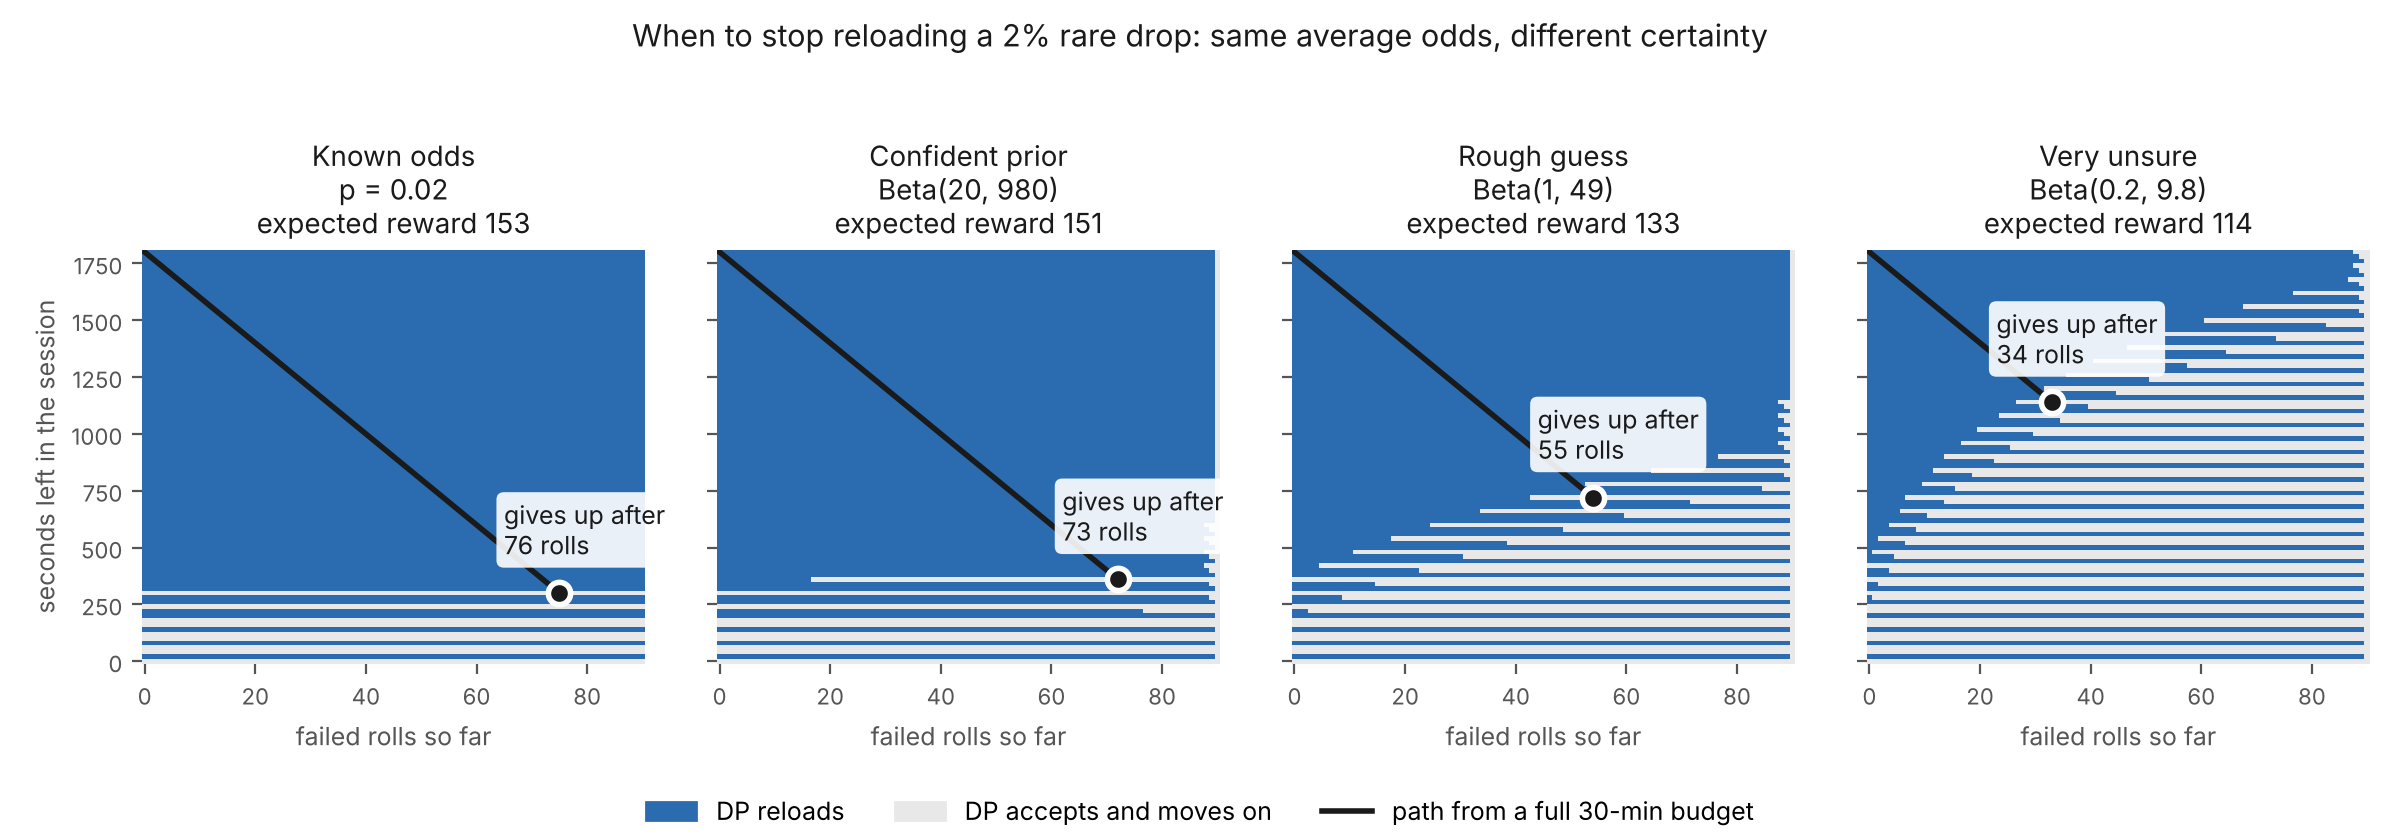
\includegraphics[width=\textwidth]{dp/out/figures/report_policy_map.png}
\caption{H5 policy maps. Blue is reload; grey is accept. The black line is the path from a full 30-minute budget. Same 2\% mean in every panel; the DP stops earlier as the prior gets weaker.}
\label{fig:H5map}
\end{figure}

\begin{figure}[H]
\centering
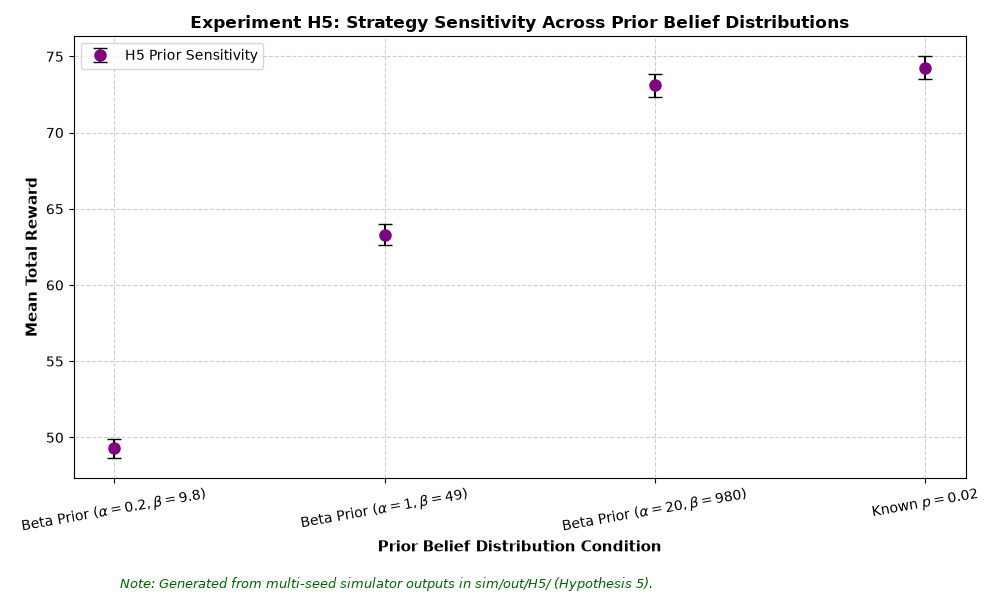
\includegraphics[width=0.92\textwidth]{analysis/experiment_h5_chart.png}
\caption{H5: DP, always-reload, and the best rare-drop-only cap.}
\label{fig:H5}
\end{figure}

\need{Yusif}{You own the H5 figure: if Fig.~\ref{fig:H5} still plots the unfair every-event \texttt{fixed\_k} bars, switch it to the rare-drop-only recheck (\texttt{dp/out/h5\_recheck.csv}).}

\subsection{Two game sessions on the same engine\who{Yera}}
\label{sec:games}
\paragraph{Pok\'emon Scarlet / Violet.}
A 60-minute shrine route, known $p = 0.08$. Odds and timings are from the Pok\'emon case file; the numbers below are the same 10,000-seed run of that file.

\begin{table}[H]
\centering
\caption{Pok\'emon SV main session, 10,000 seeds. Mean reward $\pm$ 95\% CI.}
\label{tab:pokemon}
\small
\begin{tabular}{@{}l r@{}}
\toprule
\textbf{Strategy} & \textbf{Mean reward} \\
\midrule
DP & $56.36 \pm 0.53$ \\
Always reload & $56.36 \pm 0.53$ \\
Fixed-$k = 5$ & $33.84 \pm 0.47$ \\
Reward-greedy & $32.00 \pm 0.29$ \\
Never / efficiency-greedy & $8.14 \pm 0.27$ \\
\bottomrule
\end{tabular}
\end{table}

DP equals always-reload on every seed. All four shrines have the same odds and similar reward per second, and travel ($\sim$5.5\,min) costs more than a reset ($\sim$1.5--2.5\,min), so moving on early never pays. This is H1's ``near-zero edge'' case on a real route: the simple habit is already the policy. The synthetic sweeps are where looking ahead matters.

\begin{figure}[H]
\centering
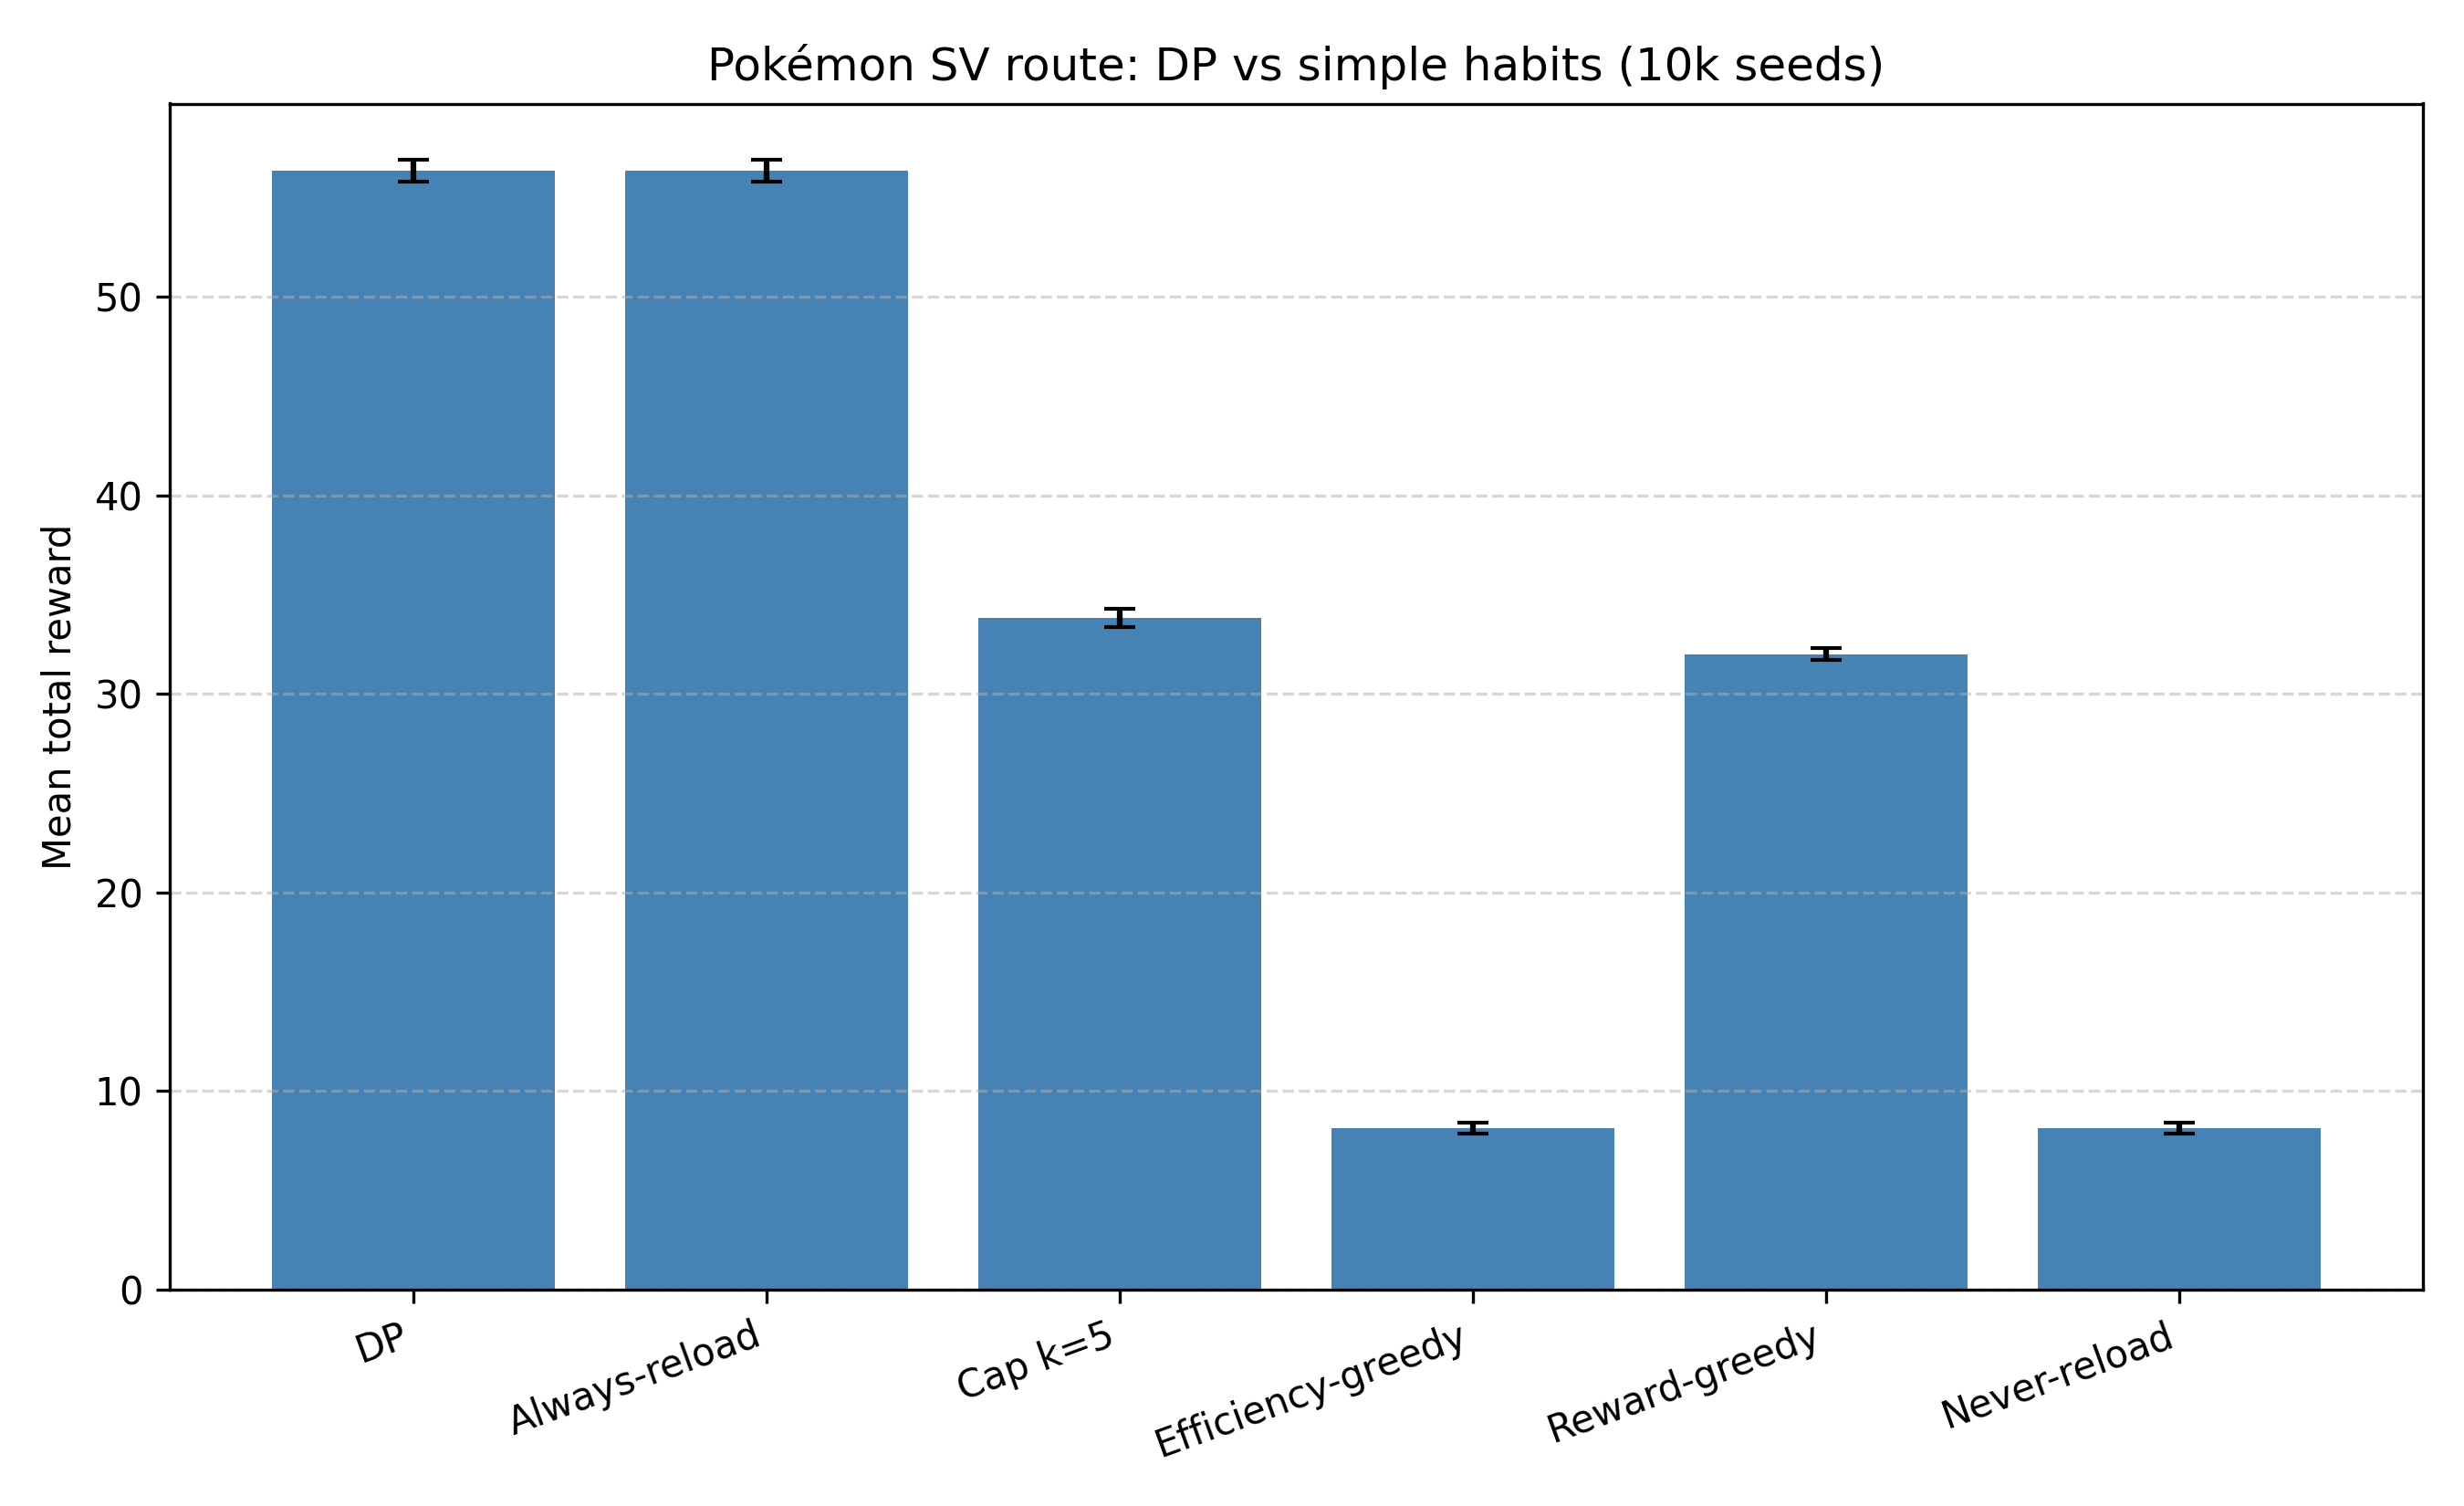
\includegraphics[width=0.88\textwidth]{analysis/experiment_pokemon_chart.png}
\caption{Pok\'emon SV main: mean reward by strategy.}
\label{fig:pokemon}
\end{figure}

\need{Roy}{One paragraph of player-facing interpretation: why nature rather than shiny, and that the 20/30/20/30 rewards are stated preferences. Sensitivity (all rewards 25) can go here or in limitations.}

\paragraph{Path of Exile Exarch contrast.}
$\mathrm{Beta}(1,49)$ on the 2\% unique; timings copied from the H5 sessions, not from footage.

\begin{table}[H]
\centering
\caption{Path of Exile Exarch Beta session, 10,000 seeds. Mean reward $\pm$ 95\% CI.}
\label{tab:poe}
\small
\begin{tabular}{@{}l r@{}}
\toprule
\textbf{Strategy} & \textbf{Mean reward} \\
\midrule
DP & $133.64 \pm 1.37$ \\
Efficiency-greedy & $119.11 \pm 1.78$ \\
Always reload & $118.03 \pm 1.79$ \\
Reward-greedy & $69.97 \pm 1.03$ \\
Fixed-$k = 5$ (every event) & $31.32 \pm 1.00$ \\
Never & $6.91 \pm 0.51$ \\
\bottomrule
\end{tabular}
\end{table}

DP beats always-reload by about $15.6$, which is the H5 $\mathrm{Beta}(1,49)$ result with Path of Exile names. Fixed-$k = 5$ here again caps every event, so it is not the H5 test; Table~\ref{tab:H5} is.

\need{Vivian}{You own the Path of Exile snapshot: add the league, snapshot date, and that the 2\% figure is a community estimate, not an official drop rate.}

\begin{figure}[H]
\centering
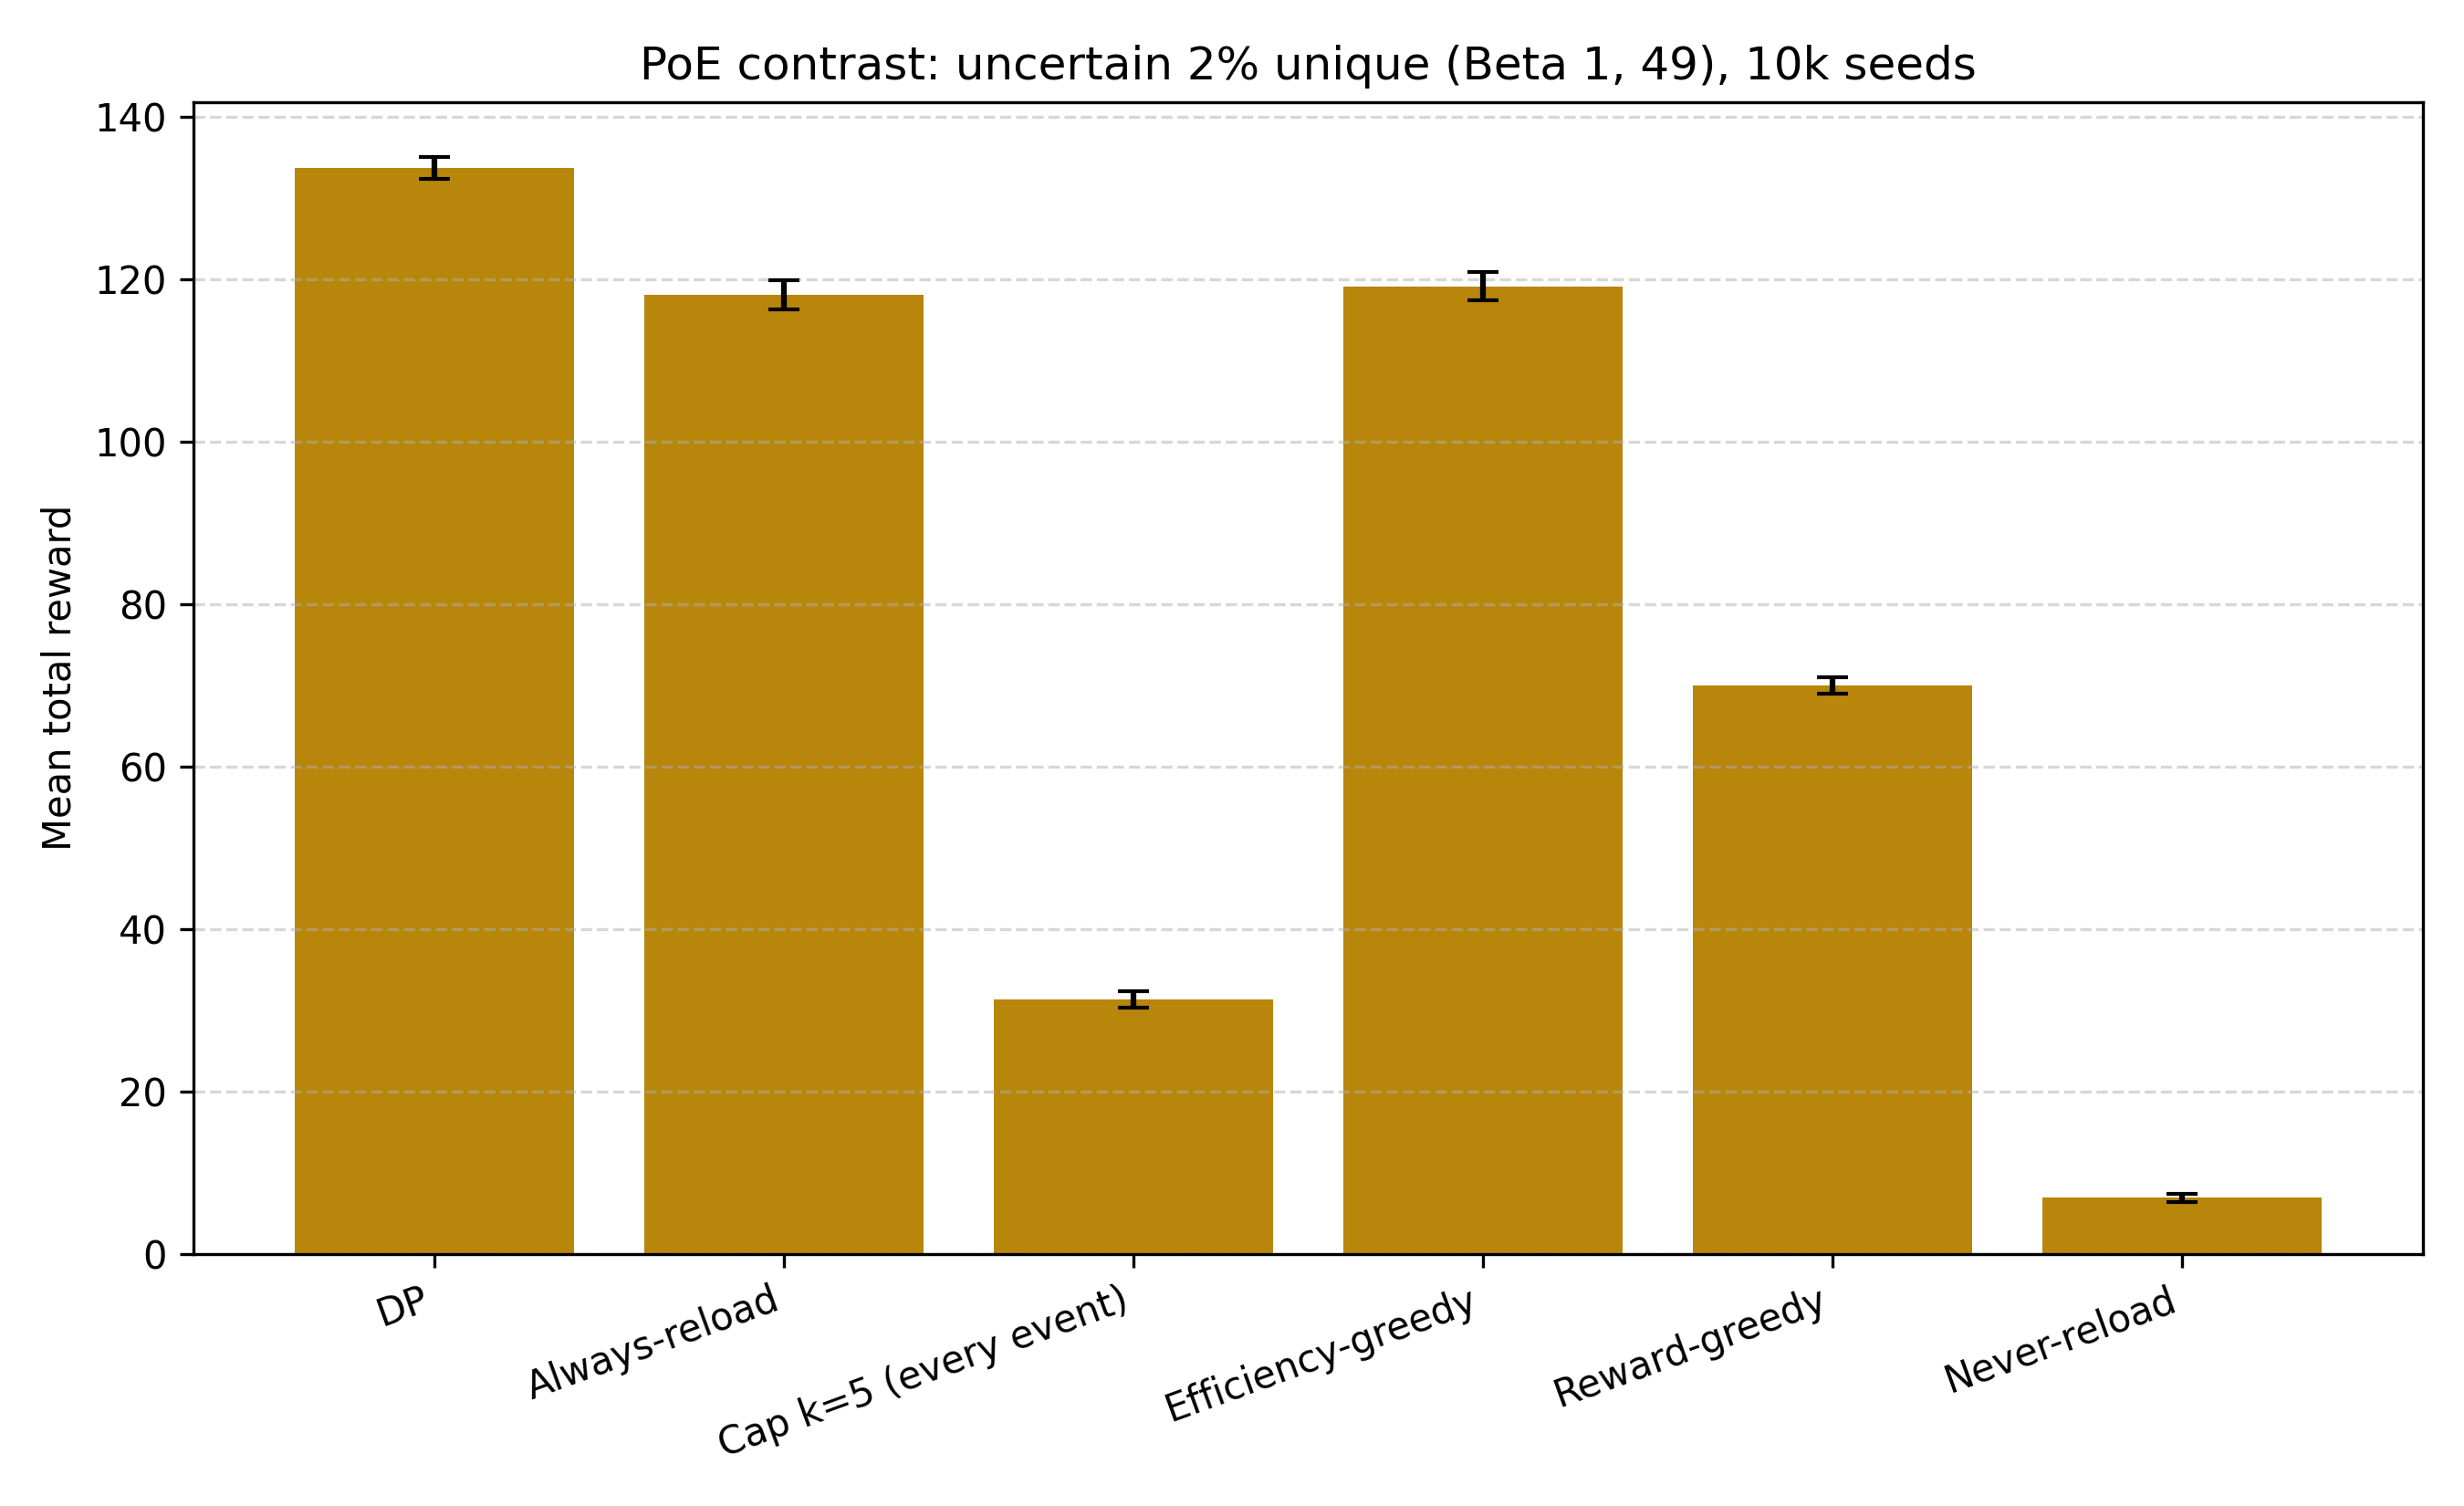
\includegraphics[width=0.88\textwidth]{analysis/experiment_poe_chart.png}
\caption{Path of Exile contrast: mean reward by strategy.}
\label{fig:poe}
\end{figure}

\subsection{What H1, H3 and H5 say together\who{Yera}}
Look ahead when time is limited and the next event is valuable enough (H1, H3), or when a failure should make you doubt the odds (H5). A constant cap is often enough if someone else has already chosen $N$. The DP is the method that produces $N$, and that switches $N$ when the later prize or the belief changes.

%======================================================================
\section{Discussion, limitations, feasibility, ethics and conclusion}
\subsection{Critical interpretation\who{Yusif}}
\need{Yusif}{Write this subsection. Points already supported by the experiment section: (1)~H1 holds on the synthetic budget sweep; (2)~H3 holds on the later-prize sweep; (3)~H5: a cap helps a little when odds are known and a lot when they are not (Table~\ref{tab:H5}); (4)~on the Pok\'emon route DP $=$ always-reload; (5)~a well-chosen cap $\approx$ DP on one uncertain event.}

\subsection{Pok\'emon reading\who{Roy}}
\need{Roy}{You own the Pok\'emon case: 3--6 sentences on whether a player would actually follow the DP, given that shrine travel dominates reset time.}

\subsection{Limitations\who{Yusif}}
\need{Yusif}{Write limitations: independent rolls; fixed event order; two illustrations do not cover every genre; H3 and H5 had to be rebuilt because the first files could not test the hypotheses.}

\need{Roy}{You own the case-study caveats: rewards are stated preferences; video timings are means from public videos, not lab measurements.}

\subsection{Feasibility\who{Yusif}}
\need{Yusif}{The prototype already runs; figures are produced from scripts; remaining work is the 10-minute talk. State runtime for 10{,}000 seeds if you have it.}

\subsection{Ethics\who{Yusif}}
\need{Yusif}{Freeze the ethics paragraph from the project plan: no surveys; public odds and public videos only; timestamps not re-uploaded footage; no live scrape, no ToS bots; no moral claim about save-scumming.}

\subsection{Future work}
\need{Yusif}{Method directions: branching routes; non-zero farm entry costs; sensitivity on the efficiency cutoff $\kappa$.}

\need{Roy}{Case-study directions: a dated Path of Exile price used as $g_i$ only if Vivian supplies it.}

\subsection{Conclusion\who{Yusif}}
\need{Yusif}{Close on the line already in the abstract: retry only when the expected gain beats the value of the same minutes later. Cite Tables~\ref{tab:H1}, \ref{tab:H3} and \ref{tab:H5}.}

%======================================================================
\section{References\who{Vivian}}
\label{sec:refs}
\need{Vivian}{You own the reference list. Check every citation against the entries below. Add Farmer and Kelly (2024) if you want it. Keep one consistent style.}

{\small
\setlength{\itemsep}{0.28em}
\begin{thebibliography}{10}
\bibitem{farmer2024}
G.~Farmer and D.~Kelly, `` `Save-scumming' in role-playing games: A call for further psychological exploration,'' British Psychological Society, Mar.\ 2024. [Online]. Available: \url{https://www.bps.org.uk/news}

\bibitem{farmer2025}
G.~Farmer, D.~Kelly and A.~Jones-Rincon, ``Save-Scumming: A Novel Exploration of Video Game Play,'' in \emph{Abstract Proceedings of DiGRA 2025: Games at the Crossroads}, 2025, doi: 10.26503/dl.v2025i3.2509.

\bibitem{farmer2026}
G.~Farmer, D.~Kelly and A.~Jones-Rincon, `` `You're playing the game wrong': Exploring motivations and perceptions of save-scumming in video games,'' PsyArXiv preprint, Jun.\ 2026, doi: 10.31234/osf.io/ew7nj\_v2.

\bibitem{luby1993}
M.~Luby, A.~Sinclair and D.~Zuckerman, ``Optimal speedup of Las Vegas algorithms,'' \emph{Information Processing Letters}, vol.~47, no.~4, pp.~173--180, 1993, doi: 10.1016/0020-0190(93)90029-9.

\bibitem{lorenz2016}
J.-H.~Lorenz, ``Completion probabilities and parallel restart strategies under an imposed deadline,'' \emph{PLOS ONE}, vol.~11, no.~10, Art.\ no.~e0164605, 2016, doi: 10.1371/journal.pone.0164605.

\bibitem{weitzman1979}
M.~L.~Weitzman, ``Optimal search for the best alternative,'' \emph{Econometrica}, vol.~47, no.~3, pp.~641--654, 1979, doi: 10.2307/1910412.

\bibitem{degroot2004}
M.~H.~DeGroot, \emph{Optimal Statistical Decisions}. Hoboken, NJ: John Wiley \& Sons, 2004, doi: 10.1002/0471729000.

\bibitem{russo2018}
D.~J.~Russo, B.~Van Roy, A.~Kazerouni, I.~Osband and Z.~Wen, ``A tutorial on Thompson sampling,'' \emph{Foundations and Trends in Machine Learning}, vol.~11, no.~1, pp.~1--96, 2018, doi: 10.1561/2200000070.

\bibitem{badanidiyuru2018}
A.~Badanidiyuru, R.~Kleinberg and A.~Slivkins, ``Bandits with knapsacks,'' \emph{Journal of the ACM}, vol.~65, no.~3, Art.\ no.~13, pp.~1--55, 2018, doi: 10.1145/3164539.

\bibitem{sargent2025}
T.~J.~Sargent and J.~Stachurski, \emph{Dynamic Programming: Finite States}. Cambridge: Cambridge University Press, 2025, doi: 10.1017/9781009540780.
\end{thebibliography}
}

%======================================================================
\section{Team contribution and generative AI}
\label{sec:contrib}

\begin{table}[H]
\centering
\caption{Team contributions. Replace the bracketed cells before submission.}
\label{tab:contrib}
\small
\renewcommand{\arraystretch}{1.15}
\begin{tabularx}{\textwidth}{@{}l l X@{}}
\toprule
\textbf{Name} & \textbf{UID} & \textbf{Contribution} \\
\midrule
Vu Q.\ Nguyen \textit{(Daniel)}
& 3036755728
& \textbf{[Daniel]} DP solver, policy maps, Beta module, H5 recheck. Confirm this sentence. \\
\addlinespace
Yerassyl Taisarinov \textit{(Yera)}
& 3036459776
& Monte Carlo simulator (\texttt{sim/}): session playback, named strategies, shared seeds, Beta hidden-$p$ draws, \texttt{sessions.csv}. Ran H1, H3, H5, Pok\'emon, and Path of Exile (10{,}000 seeds). Wrote the simulation-engine and experiment-result sections. \\
\addlinespace
Jihun Choi \textit{(Roy)}
& 3036734023
& \textbf{[Roy]} Pok\'emon event list, video timings, experiment configs. Confirm this sentence. \\
\addlinespace
Yusif Seyidov \textit{(Yusif)}
& 3036538850
& \textbf{[Yusif]} Analysis scripts, figures, report assembly, ethics. Confirm this sentence. \\
\addlinespace
Vivaan Kandhari \textit{(Vivian)}
& 3036684400
& \textbf{[Vivian]} Synthetic sessions, literature, $\rho$-baseline, Path of Exile snapshot, and the abstract through methodology draft in this file. Confirm this sentence. \\
\bottomrule
\end{tabularx}
\end{table}

\paragraph{Declaration of generative AI use.}
\begin{itemize}
\item \textbf{Yera:} none.
\item \textbf{[Daniel]} State tools used, if any, and for what (code, wording, neither).
\item \textbf{[Roy]} State tools used, if any, and for what.
\item \textbf{[Yusif]} State tools used, if any, and for what.
\item \textbf{[Vivian]} State tools used, if any, and for what.
\end{itemize}

\end{document}
